\section{2-layer NN}

There are already an elephantic number of articles on the maths behind neural networks, so I won't go into much details but rather focus on the points that are, in my view, the most important. \\

For the sake of simplicity, we will use a binary classification. Thus, the labels belong to ($\{0,1\}$). The cost function is:

$$\mathcal{L}(y, \widehat{y})=-[y\log(\widehat{y})+(1-y)\log(1-\widehat{y})]$$

We notice that the loss function decreases when $y \neq \widehat y$, which is expected as we want to penalize wrong classification.

The forward propagation allows to compute the loss functions based on the weights:

\begin{center}
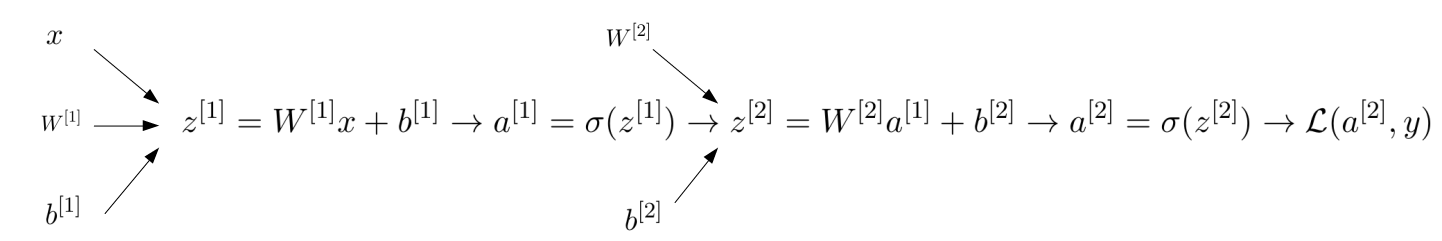
\includegraphics[scale=0.3]{img/NN_2.png}
\end{center}

As we can see here, we use two sets of weights and biases: $W^{[1]}$, $b^{[1]}$, $W^{[2]}$ and $b^{[2]}$. \\

Then, the backward propagation allows to find how to update the weights in order to minimize the loss:

\begin{center}
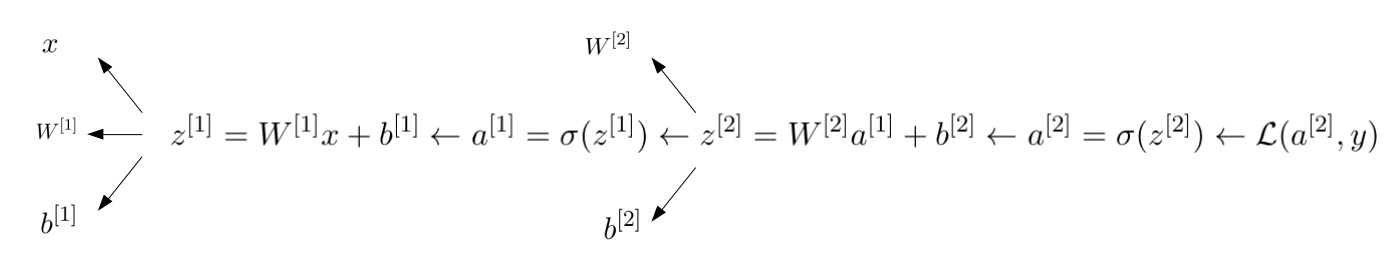
\includegraphics[scale=0.3]{img/NN_2_backward.png}
\end{center}

For the full details on the derivative computation, I explain everything on \href{https://savoga.github.io/machinelearning/neural-network/}{my website} (hopefully I didn't do too many mistakes).